\chapter{Решение} \label{chapt3}

\section{Получение данных} \label{sect3_1}
Для решения задачи классификации нейронной сетью требуется наличие данных для обучения. Датасетов с настоящей проблемой в открытом доступе не нашлось, поэтому данные пришлось получать вручную.

\begin{figure}[ht] 
  \center
  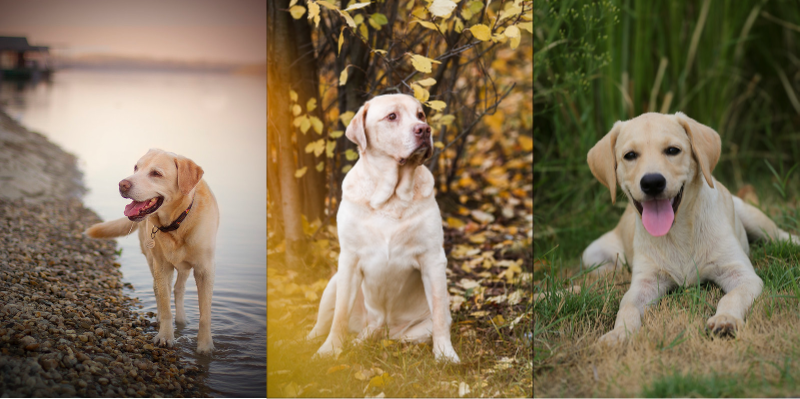
\includegraphics [width=\textwidth*2/3] {dogs-classes}
  \caption{Позы собаки, на которые классифицируются изображения: собака стоит, собака сидит и собака лежит} 
  \label{img:classes}  
\end{figure}

\subsection{Первая итерация} \label{subsect3_1_1}
За основу был взят датасет OpenImageDataset[2] - набор изображений на более чем тысячу разных классов. Из него был взят подкласс Dog, в котором было 20000 изображений собак. Далее эти данные были размечены на Яндекс.Толоке. Каждое изображение было показано пользователю Толоки с вопросом “В какой позиции собака находится на этом фото”. Фотографии были размечены с пятикратным перекрытием, т.е. каждое изображение размечалось пять раз разными людьми.
На выходе получился скромного размера датасет, часть изображений в нём не подходили под постановку задач, но на выходе имелась следующая информация:
\begin{enumerate}
    \item Поза собаки (стоит, сидит, лежит на спине, лежит на боку)
    \item Поза хвоста собаки (вверх, вниз, прямо)
    \item Рот собаки (открыт, закрыт, высунут язык)
    \item Уши собаки (торчат, опущены)
    \item Количество собак в кадре
    \item Загорожена ли собака в кадре
    \item Ограничивающая рамка (bounding box) вокруг собаки.
    \item Ограничивающая рамка ушей, хвоста и рта собаки.
\end{enumerate}

\subsection{Создание эталонного датасета} \label{subsect3_1_2}
Учитывая прошлые ошибки было принято решение собрать датасет заново, используя опыт, полученный при разметке первого.

Главные изменения заключаются в следующем:
\begin{enumerate}
    \item Датасет собирается итеративно по небольшим частям и выводы делаются сразу
    \item Размер каждого класса удерживается на одинаковом уровне
    \item Проводится учёт всех изображений, которые тяжело размечать
\end{enumerate}{}

В статье Amy Bearman и Cathering Dong \cite{Bearman2015HumanPE} указывается что нейронным сетям тяжело распознать позу, при наличии окклюзий, поворотов и переворотов, сильных перспективных искажений, и множественных объектов. В новом датасете было уделено особое внимание трудноклассифицируемым изображениям, поэтому они всячески избегались.

\begin{figure}[ht] 
  \center
  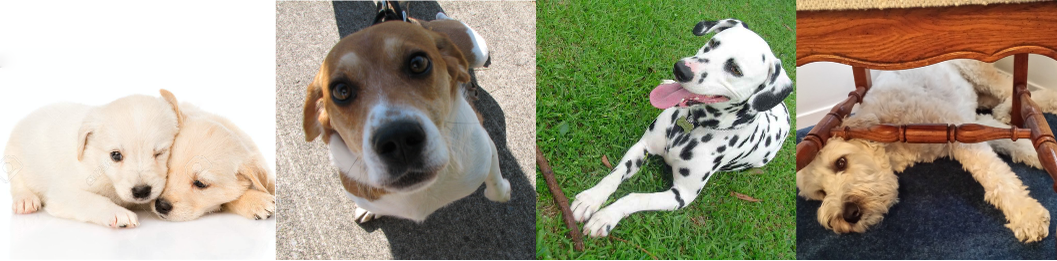
\includegraphics [width=\textwidth] {hazards_dogs}
  \caption{Позы, которые трудно определить: множественные объекты, перспективные искажения, повороты и окклюзии} 
  \label{img:hazards_dogs}  
\end{figure}

На этот раз источником изображений был Flickr. В нём содержится множество фотографий, который можно было фильтровать как по ориентации - только вертикальные, например. По породе - можно явно указать, что мы ищем Лабрадора Ретривера. Либо только снятые на телефон. В общем, сильно больше контроля при выборе фотографий.

В итоге были собраны изображения собак по 100 изображений на целевой класс. На них была обучена простейшая архитектура, т.н. ShallowNet с одним свёрточным слоем.
Результаты следующие:
\begin{itemize}
    \item При классификации «в лоб» достигается точность в 60\%
    \item При обрезании изображений по ограничительной рамке собаки, точность увеличивается до 68\%
    \item При использовании черно-белых изображений точность также возрастает до 68\%
\end{itemize}

\subsection{Фильтрация исходного датасета} \label{subsect3_1_2}
Собирать фотографии заново было достаточно хорошим упражнением, но главной проблемой были огромные временные затраты на создание датасета даже с 300 фотографиями. Более того, из 80000 фотографий по тегу Лабрадор Ретривер, автором и его ассистентом было просмотрено 70000 из них. И уже из них были собраны те 300 фотографий.
В итоге было принято решение просмотреть исходный датасет и повысить точность самих данных, это достаточно просто, ведь в датасете, исходя из качества в 70\%, присутствует около 15\% проблемных фотографий, которые достаточно удалить из коллекции чтобы повысить качество.

\section{Проверка задачи на решаемость} \label{sect3_2}
После сбора данных, была предпринята попытка обучить нейронную сеть классифицировать полученные изображения. В лоб эта задача решается тяжело, из-за низкого качества входных данных и изначально малой обучающей выборки. Поэтому пришлось работать с обучающей выборкой. Были предприняты следующие меры для улучшения работы системы.
\begin{itemize}
    \item Все изображения были обрезаны по ограничивающей рамке собаки. И это дало сильный прирост в качестве классификации, 55\% -> 65\% на 5 классах
    \item Дополнительно были размечены изображения, где собака видна плохо, и были удалены из выборки. Это сократило размер и без того маленькой выборки, не сильно улучшив данные, т.к. качество разметки на Толоке достаточно низкое.
    \item Добавлены аугментации обучающей выборки. Аугментации позволяют нейронной сети не запоминать обучающие данные точь-в-точь, что снижает её способность к переобучению. Добавило около 2\% точности, 65-67\%
    \item Проведена очистка изображений. Из обучающей выборки были исключены изображения с несколькими собаками и собаками, которых не видно целиком. Это дало ощутимый прирост, но обучающая выборка сократилась до недопустимо маленьких размеров. Добавлено около 3\% точности, 67\%->69\%
    \item Использование transfer learning (переносимость обучения) - все модели, которые использовались здесь, не обучались с нуля. Они обучались на нейронной сети, уже предобученной классифицировать 1000 классов ImageNet(другого открытого датасета с изображениями).

\end{itemize}

